\documentclass{article} % For LaTeX2e
\usepackage{nips15submit_e,times}
\usepackage{hyperref}
\usepackage{url}
%\documentstyle[nips14submit_09,times,art10]{article} % For LaTeX 2.09
\usepackage{amsmath}
\usepackage{graphicx}
\usepackage{listings}
\usepackage{subfig}
\title{Logistic and Softmax Regression for Handwritten Digits Classification}


\author{
Shilin Zhu \\
Ph.D. student, Computer Science\\
UCSD\\
La Jolla, CA \\
\texttt{shz338@eng.ucsd.edu} \\
\And
Yunhui Guo\\
Ph.D. student, Computer Science\\
UCSD\\
La Jolla, CA \\
\texttt{yug185@eng.ucsd.edu} \\
}

% The \author macro works with any number of authors. There are two commands
% used to separate the names and addresses of multiple authors: \And and \AND.
%
% Using \And between authors leaves it to \LaTeX{} to determine where to break
% the lines. Using \AND forces a linebreak at that point. So, if \LaTeX{}
% puts 3 of 4 authors names on the first line, and the last on the second
% line, try using \AND instead of \And before the third author name.

\newcommand{\fix}{\marginpar{FIX}}
\newcommand{\new}{\marginpar{NEW}}

\nipsfinalcopy % Uncomment for camera-ready version

\begin{document}
\maketitle

\section{Abstract}
In this report, we will introduce how to use logistic regression and softmax regression to do handwritten digits classification. We did extensive experiments on the MNIST datasets [2]. For 2-way classification, we can achieve an accuracy of $98\%$ if the targets are digit `2' and digit `3' and we can achieve an accuracy of $97\%$ if the targets are digit `2' and digit `8' by using logistic regression. For 10-way classification for all 10 digits, we can achieve an accuracy  of $93.55\%$ by using softmax regression.

\section{Logistic Regression via Gradient Descent}

\subsection{Problem Definition}
In this work, we realize the handwritten digit classification using MNIST database. Our goal is to accurately and robustly recognize what number is present in a new image. In this section we will first use logistic regression to classify only two digit classes (binary classification), later in the next section we will use softmax regression to generalize logistic regression into $N$ classes.

\subsection{Mathematical Derivation and Methods}
\textbf{Derive the gradient for logistic regression:} \\
The cross-entropy cost function can be expressed as

\begin{equation}
	E(w) = - \frac{1}{N}\sum_{n=1}^{N}[t^{n}\ln(y^{n})+(1-t^{n})\ln(1-y^{n})]
\end{equation}

where $t^{n}$ is the target label for example $n$ and $y^{n}$ is our prediction for this example. To perform gradient descent, we need to first compute the gradient (derivative) of the cost function with respect to the parameters. The gradient of cost function on example $n$ is

\begin{equation}
	-\frac{\partial E^{n}(w)}{\partial w_{j}} = \frac{1}{N}\frac{\partial [t^{n}\ln(y^{n})+(1-t^{n})\ln(1-y^{n})]}{\partial w_{j}} 
\end{equation}

where $y^{n}$ is the prediction of logistic regression as

\begin{equation}
	y^{n} = g(\sum_{j=0}^{m}w_{j}x_{j}^{n})
\end{equation}

and $g(\cdot)$ is the sigmoid activation function and its derivative is

\begin{equation}
	g^{\prime}(z^{n}) = \frac{d(\frac{1}{1+e^{-z^{n}}})}{dz^{n}} = g(z^{n})(1-g(z^{n}))
\end{equation}

where $z ^{n}= \sum_{j=0}^{m}w_{j}x_{j}^{n}$. According to the chain rule in calculus, we can then compute the gradient (derivative) of the cost function on example $n$ with respect to the parameters as

\begin{equation}
	-\frac{\partial E^{n}(w)}{\partial w_{j}} = -\frac{\partial E^{n}(w)}{\partial y^{n}}\frac{\partial y^{n}}{\partial z^{n}}\frac{\partial z^{n}}{\partial w_{j}} = \frac{1}{N}(\frac{t^{n}}{y^{n}}-\frac{1-t^{n}}{1-y^{n}})\cdot y^{n}(1-y^{n})\cdot x_{j}^{n} = \frac{1}{N}(t^{n}-y^{n})x_{j}^{n}
\end{equation}

Note that we can always add a factor of $1/N$ to scale the cost and gradient to somehow speed up the learning, and this will not change the optimization results (learned parameters).

\subsection{Data Reading, Parsing and Feature Extraction} 
In this work we use the famous MNIST hand written digits database created by Yann LeCun. Each image in the database contains $28 \times 28$ pixels and each pixel has a grayscale intensity, so that the input feature $x \in R^{784}$ after we unroll the 2D image into an 1D vector. To include the bias term, after reading the data, we append a '1' to the beginning of each $x$ vector so the final $x \in R^{785}$. We will use the first 20,000 training images and the last 2,000 test images. Note that for logistic regression to do binary classification, we can only use the images of two specific digit classes, so that the actual training images and test images are smaller than 20,000 and 2,000 respectively. To speed up learning, we need to apply feature normalization. For images, the most common way is to normalize the pixel values by the maximum pixel value 255. After normalization, all the values in $x$ is now ranging from 0 to 1.

The following code shows how we can choose the example images corresponding to two specific digit classes. For the rest of the report, we choose two binary classification problems: 2 vs. 3 and 2 vs. 8.

\subsection{Experimental Results and Discussion}
\textbf{Batch gradient descent}\\
We first apply batch gradient descent rule on logistic regression since the training set is not that huge, thus batch gradient descent can work reasonably fast. 

\begin{figure}%
	\centering
	\subfloat[Cost function with iterations for batch GD on classifying 2 vs. 3]{{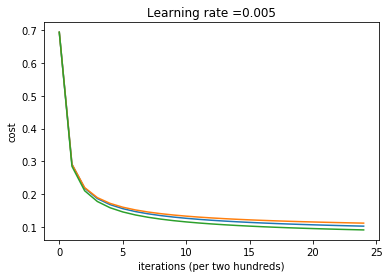
\includegraphics[width=2.5in]{images/P1_2.png}  }}%
	\qquad
	\subfloat[Cost function with iterations for batch GD on classifying 2 vs. 8]{{	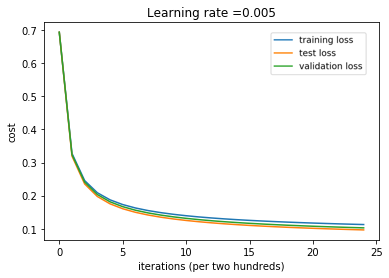
\includegraphics[width=2.5in]{images/P1.png}  }}%
	\caption{Cost function through batch GD training process}%
	\label{fig:P1}%
\end{figure}

\begin{figure}%
	\centering
	\subfloat[Cost function with iterations for mini-batch GD on classifying 2 vs. 3]{{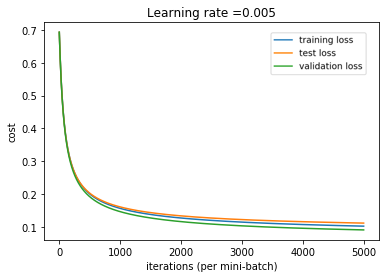
\includegraphics[width=2.5in]{images/P2_2.png}  }}%
	\qquad
	\subfloat[Cost function with iterations for mini-batch GD on classifying 2 vs. 8]{{	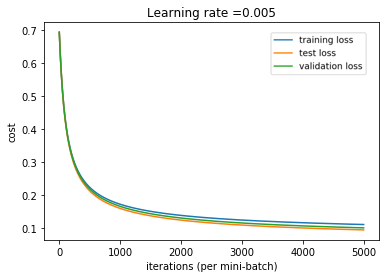
\includegraphics[width=2.5in]{images/P2.png}  }}%
	\caption{Cost function through mini-batch GD training process}%
	\label{fig:P2}%
\end{figure}

After trying different values of learning rate, we found $0.005$ is a reasonably good learning rate for this problem. Fig. \ref{fig:P1} plots the  loss function over training for the training set, the hold-out validation set and the test set. From the results we can see the model tries to minimize the cost and meanwhile maximize the likelihood to perform good prediction on the data. Here for both 2 vs. 8 and 3 vs. 8 cases, the test set accuracies are both around $97\%$ so our model generalizes reasonably well given this large dataset used for the training, as shown in Fig. \ref{fig:P3}.

\textbf{Mini-Batch gradient descent}\\
We can use mini-batch gradient descent to speed up learning process. Since the one-step optimization is done on a smaller mini-batch, the cost function will not monotonically decrease as batch gradient descent. Here we change the weights after a mini-batch of roughly $10\%$ of the entire training set. This set of mini-batch size can result in relatively smooth curve of the cost function. Fig. \ref{fig:P2} plots the loss function over training for consecutive mini-batches. Since the validation set always has very similar errors as the test set, we can conclude the hold-out set work as a good stand-in for the test set and their underlying data distributions are same.

\textbf{Accuracy of Prediction Using Logistic Regression Classifier}\\

\begin{figure}%
	\centering
	\subfloat[Accuracy with iterations on classifying 2 vs. 3]{{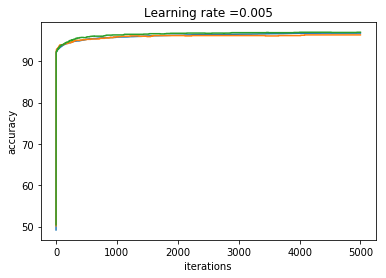
\includegraphics[width=2.5in]{images/P3_2.png}  }}%
	\qquad
	\subfloat[Accuracy with iterations on classifying 2 vs. 8]{{	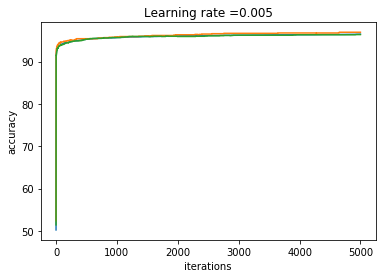
\includegraphics[width=2.5in]{images/P3.png}  }}%
	\caption{Accuracy through training process}%
	\label{fig:P3}%
\end{figure}

\textbf{Weight Visualization}\\
We can visualize the weights learned to see what logistic regression learns through the training process. Fig. \ref{fig:P4} shows that the model indeed learn the representation of numbers we want it to learn. The neurons are activated and de-activated based on the structure of the handwritten digit. And since the cost function is cross-entropy loss, which means the maximum likelihood corresponds to the maximum prediction. In order to achieve maximum prediction value which is the inner product of input $X$ and weights, the angle between these two vectors in the feature space should be zero so that their inner product is maximized. Thus the weights look very similar to $X$ in the feature space and so as our 2-D visualization.
\begin{figure}%
	\centering
	\subfloat[Weights learned on classifying 2 vs. 3]{{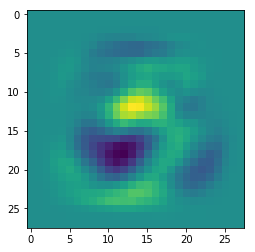
\includegraphics[width=1.5in]{images/P4_2.png}  }}%
	\qquad
	\subfloat[Weights learned on classifying 2 vs. 8]{{	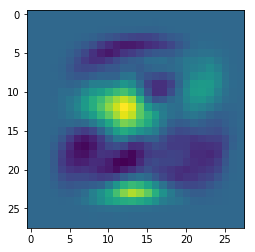
\includegraphics[width=1.5in]{images/P4.png}  }}%
	\qquad
	\subfloat[Difference of the weights between the two classifiers]{{	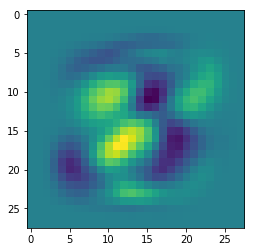
\includegraphics[width=1.5in]{images/P5.png}  }}%
	\caption{Weight visualization on binary classification using logistic regression}%
	\label{fig:P4}%
\end{figure}

Computing the difference between these two different classifiers, we can get a new weight matrix visualized in Fig. \ref{fig:P4}. This result shows that the new weights can be used to accurately classify digit 3 and digit 8 since the neurons will be activated and de-activated based on these new weights.


In the next part of this section, we are going to add regularization to our model and analyze it via experiments.

\subsection{Derive the gradient for regularized logistic regression:}

To prevent potential overfitting, regularization is used in logistic regression. The cross-entropy cost function with regularization term can be computed as

\begin{equation}
	E(w) = - \frac{1}{N}\sum_{n=1}^{N}[t^{n}\ln(y^{n})+(1-t^{n})\ln(1-y^{n})] + \lambda * C(w)
\end{equation}

where $C(w)$ represents the complexity of the model. $L1$ and $L2$ regularizations are two most common functions people use

\begin{equation}
	C(w) = ||w||^{2} = \sum_{i, j}w_{i, j}^{2}, \text{if use $L_2$ regularization}
\end{equation}

\begin{equation}
	C(w) = |w| = \sum_{i, j}|w_{i, j}|, \text{if use $L_1$ regularization}
\end{equation}

Thus the gradient of cost function on example $n$ is 

\[
    -\frac{\partial E^{n}(w)}{\partial w_{j}} = 
\begin{cases}
    \frac{1}{N}(t^{n}-y^{n})x_{j}^{n} - 2\lambda w_{j},& \text{if use $L_2$ regularization}\\
    \frac{1}{N}(t^{n}-y^{n})x_{j}^{n} - \lambda sign(w_{j}), & \text{if use $L_1$ regularization}
\end{cases}
\]

where $sign(w_{j})$ is the signature function of $w_{j}$. 

Note that we can always add a factor of $1/N$ to scale the cost and gradient to somehow speed up the learning, and this will not change the optimization results (learned parameters).

\begin{figure}%
	\centering
	\subfloat[Accuracy when lambda = 0.1 using L1 regularization]{{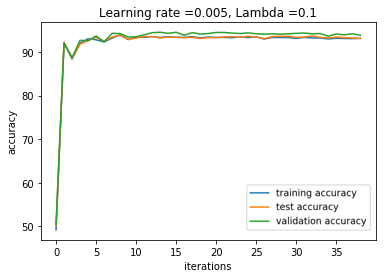
\includegraphics[width=1.5in]{images/P7.png}  }}%
	\qquad
	\subfloat[Accuracy when lambda = 0.03 using L1 regularization]{{	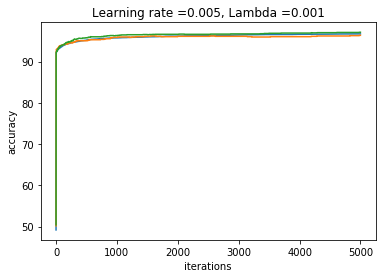
\includegraphics[width=1.5in]{images/P7_2.png}  }}%
	\qquad
	\subfloat[Accuracy when lambda = 0.01 using L1 regularization]{{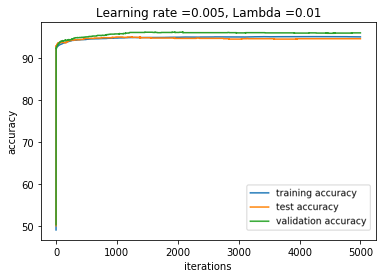
\includegraphics[width=1.5in]{images/P7_3.png}  }}%
	\qquad
	\subfloat[Accuracy when lambda = 0.003 using L1 regularization]{{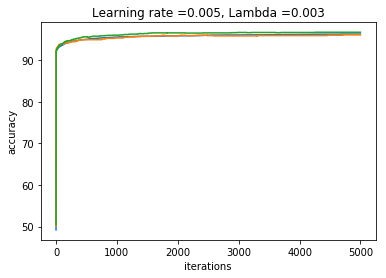
\includegraphics[width=1.5in]{images/P7_4.png}  }}%
	\qquad
	\subfloat[Accuracy when lambda = 0.001 using L1 regularization]{{	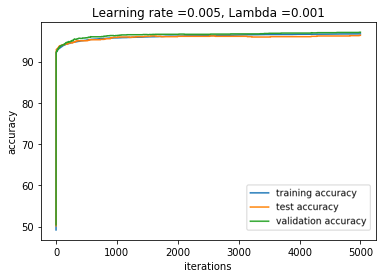
\includegraphics[width=1.5in]{images/P7_5.png}  }}%
	\qquad
	\subfloat[Accuracy when lambda = 0.0001 using L1 regularization]{{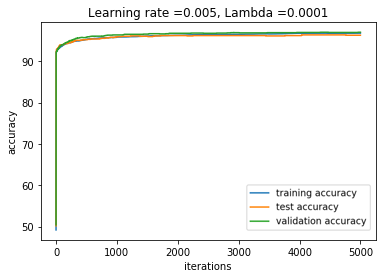
\includegraphics[width=1.5in]{images/P7_7.png}  }}%
	\caption{Accuracy using L1 regularization}%
	\label{fig:P7}%
\end{figure}

\textbf{Tuning the Regularization Parameter}\\
In order to choose a reasonably good regularization model, we need to tune the regularization parameter and choose the one which results in the best accuracy on the hold-out validation set. Here we try three values for regularization parameter $\lambda$: 0.0001, 0.001 and 0.01. Fig. \ref{fig:P7} and Fig. \ref{fig:P8} show the results with different $\lambda$ on L1 and L2 regularization. From the experimental results we can see as soon as we do not set $\lambda$ too large, we can always get reasonably well performance (so the performance is not very sensitive to the regularization strength) if we are training our model using a large enough dataset. 

If we set lambda very large as shown in Fig. \ref{fig:P11}, we can see that L1 regularization will be over strong and cause the model fail to converge and may experience underfit problem. L2 regularization is more robust against large $\lambda$ compared to L1 regularization.

\begin{figure}%
	\centering
	\subfloat[Accuracy when lambda = 0.1 using L2 regularization]{{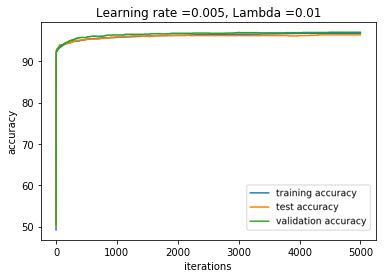
\includegraphics[width=1.5in]{images/P8.png}  }}%
	\qquad
	\subfloat[Accuracy when lambda = 0.03 using L2 regularization]{{	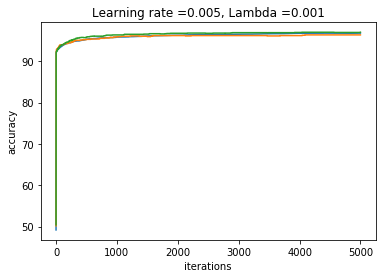
\includegraphics[width=1.5in]{images/P8_2.png}  }}%
	\qquad
	\subfloat[Accuracy when lambda = 0.01 using L2 regularization]{{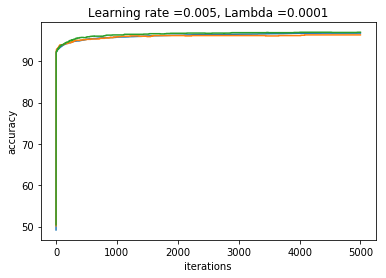
\includegraphics[width=1.5in]{images/P8_3.png}  }}%
	\qquad
	\subfloat[Accuracy when lambda = 0.003 using L2 regularization]{{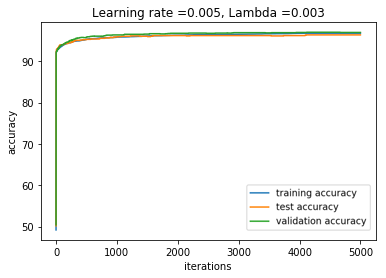
\includegraphics[width=1.5in]{images/P8_4.png}  }}%
	\qquad
	\subfloat[Accuracy when lambda = 0.001 using L2 regularization]{{	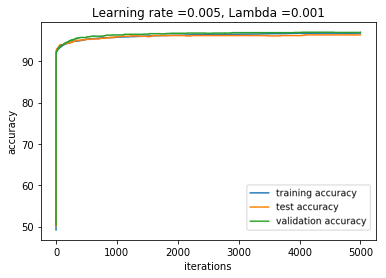
\includegraphics[width=1.5in]{images/P8_5.png}  }}%
	\qquad
	\subfloat[Accuracy when lambda = 0.0001 using L2 regularization]{{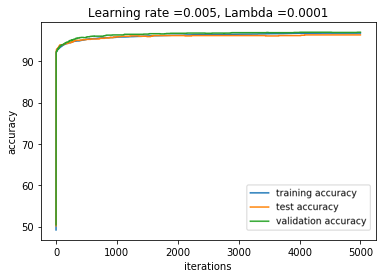
\includegraphics[width=1.5in]{images/P8_7.png}  }}%
	\caption{Accuracy using L2 regularization}%
	\label{fig:P8}%
\end{figure}

\begin{figure}%
	\centering
	\subfloat[Accuracy when lambda = 1 using L1 regularization]{{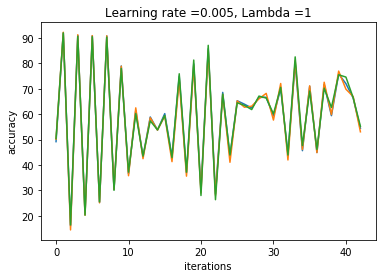
\includegraphics[width=2.5in]{images/P11.png}  }}%
	\qquad
	\subfloat[Accuracy when lambda = 1 using L2 regularization]{{	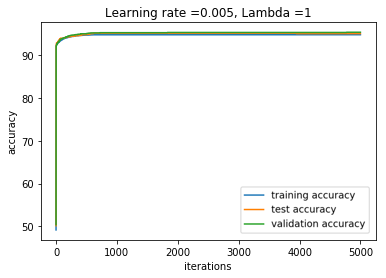
\includegraphics[width=2.5in]{images/P11_2.png}  }}%
	\caption{Setting up lambda to be very large values}%
	\label{fig:P11}%
\end{figure}

\textbf{Reality Check on the Length of Weight Vector}\\
Fig. \ref{fig:P4} shows the experimental results using L1 and L2 regularization. From the figures we can see that stronger regularization will result in smaller weights since the regularization penalizes large weights. This is consistent with the mathematics of our cost function since if we use a very large $\lambda$, the optimizer will pay more attention to minimize the regularization term instead of minimizing the loss between the prediction and the ground truth labels. 

\begin{figure}[h]%
	\centering
	\subfloat[Length of weight vector using L1 regularization]{{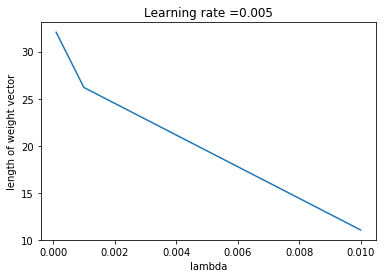
\includegraphics[width=2.5in]{images/P6.png}  }}%
	\qquad
	\subfloat[Length of weight vector using L2 regularization]{{	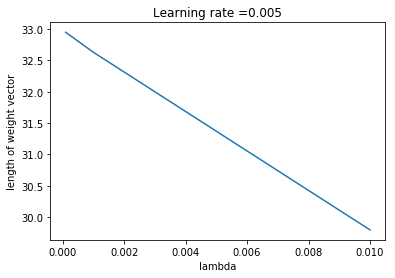
\includegraphics[width=2.5in]{images/P6_2.png}  }}%
	\caption{Reality check on the length of the weight vector}%
	\label{fig:P4}%
\end{figure}

\textbf{Final Test Set Error with Regularization}\\
We also plot the final test set error with different values of the regularization parameter, as shown in Fig. \ref{fig:P9}. For L1 regularization we can see that when $\lambda$ is relatively small, the test accuracy will increase as we increase $\lambda$. This proves that regularization can sometimes make the model generalize better. In this example the performance improvement is very small since the training dataset is reasonably large and with good quality, so that overfitting is not a great issue anymore. We can also observe that when $\lambda$ is getting larger and larger, the test accuracy actually decreases (as well as on the training and validation set). This is because although strong regularization makes the model generalize well, over strong regularization will cause the model to be too simple and cannot even fit the data very well (as shown in Fig. \ref{fig:P11}). But we can conclude that using $\lambda$ between 0.0001 and 0.001 can all work reasonably well for L1 and L2 regularized model. For L2 regularization, it is more robust and less sensitive as we change $\lambda$ compared with L1 regularization.

\begin{figure}%
	\centering
	\subfloat[Final test accuracy using L1 regularization]{{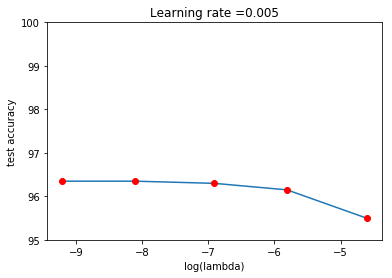
\includegraphics[width=2.5in]{images/P9.png}  }}%
	\qquad
	\subfloat[Final test accuracy using L2 regularization]{{	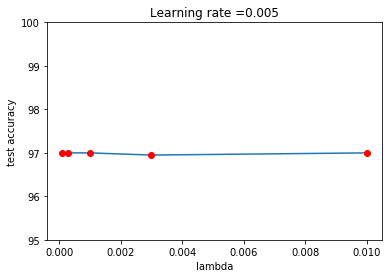
\includegraphics[width=2.5in]{images/P9_2.png}  }}%
	\caption{Final test accuracy using regularization}%
	\label{fig:P9}%
\end{figure}

\textbf{Weight Visualization with Regularization}\\
We further visualize the weights learned with our regularized model, which are shown in Fig. \ref{fig:P10}. From the results we can see that when $\lambda$ increases, the learned parameters (weights) become simpler and cannot represent the data very well since we cannot see the structure of the digits anymore under the case with too large $\lambda$. But when $\lambda$ is set a good enough value, then they can learn the structure and distribution of the data quite well. From this result we can also see that L2 regularization is less sensitive as we change $\lambda$ compared with L1 regularization since L2 regularization can still make the model to learn good representations even if $\lambda$ is large.

To conclude, our logistic regression classifier is well trained and can be generalized to predict on test data very well. Using cross-entropy cost function as the optimization objective, we can visualize the weights which reflect the structure of the digits. Regularization can be applied to the model and choosing a good $\lambda$ is critical for the classifier. For large training datasets, the overfitting is not an issue with complex models. Since the logistic classifier only has one output unit, to classify all the 10 digits we need to use multiple output units where softmax regression is useful.

\begin{figure}%
	\centering
	\subfloat[Weights when lambda = 0.1 using L1 regularization]{{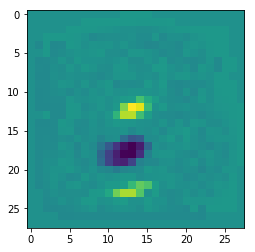
\includegraphics[width=1.0in]{images/P10_7.png}  }}%
	\qquad	
	\subfloat[Weights when lambda = 0.01 using L1 regularization]{{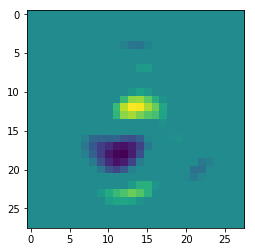
\includegraphics[width=1.0in]{images/P10.png}  }}%
	\qquad
	\subfloat[Weights when lambda = 0.001 using L1 regularization]{{	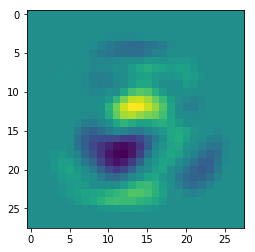
\includegraphics[width=1.0in]{images/P10_2.png}  }}%
	\qquad
	\subfloat[Weights when lambda = 0.0001 using L1 regularization]{{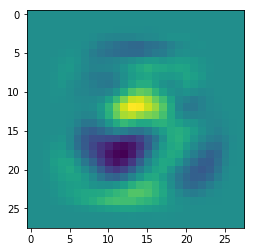
\includegraphics[width=1.0in]{images/P10_3.png}  }}%
	\qquad
	\subfloat[Weights when lambda = 0.1 using L2 regularization]{{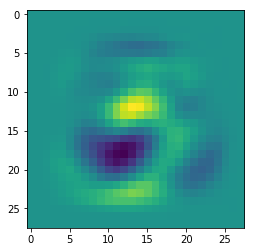
\includegraphics[width=1.0in]{images/P10_8.png}  }}%
	\qquad	
	\subfloat[Weights when lambda = 0.01 using L2 regularization]{{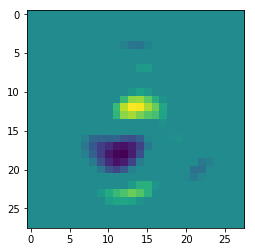
\includegraphics[width=1.0in]{images/P10_4.png}  }}%
	\qquad
	\subfloat[Weights when lambda = 0.001 using L2 regularization]{{	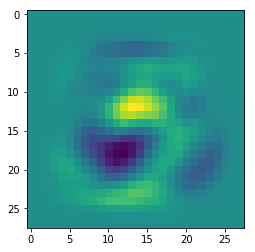
\includegraphics[width=1.0in]{images/P10_5.png}  }}%
	\qquad
	\subfloat[Weights when lambda = 0.0001 using L2 regularization]{{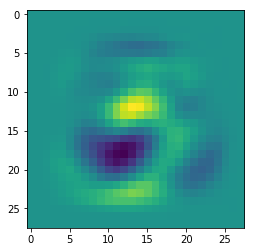
\includegraphics[width=1.0in]{images/P10_6.png}  }}%
	\caption{Weights visualization using regularization}%
	\label{fig:P10}%
\end{figure}

\newpage
\section{Softmax Regression via Gradient Descent}
\subsection{Problem definition}
In this problem, we need to classify MNIST datasets using softmax regression. In the experiments, we only use the first 20,000 training images and the last 2,000 test images.

\subsection{Methods}
\textbf{Derive the gradient for Softmax Regression:} \\
The cross entropy cost function can be expressed as,

\begin{equation}
	E = \sum_{n=1}^{N}\sum_{k=1}^{c}t_k^n\ln y_k^n
\end{equation}

Where, 
\begin{equation}
	y_k^n = \frac{\exp{(a_k^n)}}{ \sum_{k'}\exp{(a_{k'}^n})}
\end{equation}
And, 
\begin{equation}
	a_k^n = w_k^Tx^n
\end{equation}


We can calculate the gradient for softmax regression as follows,
\begin{equation}
\begin{split}
-\frac{\partial E^n(w)}{\partial w_{jk}}& = - \frac{\partial E^n(w)}{\partial a_k^n}\frac{\partial a_k^n}{\partial w_{jk}} \\
& = -\sum_{k'} \frac{\partial E^n(w)}{\partial y^n_{k'}} \frac{\partial y^n_{k'}}{\partial a^n_k}\frac{\partial a_k^n}{\partial w_{jk}} \\
\end{split}
\end{equation}
And 
\begin{equation}
\begin{split}
\frac{\partial y^n_{k'}}{\partial a^n_k} &=
\frac{\partial \frac{\exp{(a^n_{k'})}}{ \sum_{k'}\exp{(a_{k'}^n})}}{\partial a^n_k} \\
& = y^n_{k'}\delta_{kk'} - y^n_{k
'}y^n_{k}\\
\end{split}
\end{equation}
Where $\delta_{kk} = 1$ if $k = k'$, otherwise $\delta_{kk} = 0$.
And
\begin{equation}
\begin{split}
	\frac{\partial E^n(w)}{\partial y^n_{k'}} = \frac{t^n_{k'}}{y^n_{k'}}
\end{split}
\end{equation}
Substitute Equation (5) and Equation (6) into Equation (4) we get,
\begin{equation}
\begin{split}
	-\frac{\partial E^n(w)}{\partial w_{jk}} = (t^n_k - y^n_k)x_j^n 
\end{split}
\end{equation}
\textbf{Derive the gradient for Softmax Regression with Regularizations:} \\

With regularization, generally the loss function can be writen as,
\begin{equation}
J(w) = E(w) + \lambda C(w)
\end{equation}
If we use $L_1$ regularization in softmax regression,
\begin{equation}
	\lambda C(w) = \lambda C_{L_1}(w) =   \lambda \sum_{j,k}|w_{jk}|
\end{equation}

We can compute the derivate of $\frac{\partial C}{\partial w}$ as follows,
\begin{equation}
	\frac{\partial C_{L_1}(w)}{\partial w_{jk}} = sign(w_{jk})
\end{equation}
Where $sign(x) = 1$ if $x > 0$, $sign(x) = 0$ if $x = 0$ and $sign(x) = -1$ if $x < 0$.

If we use $L_2$ regularization in softmax regression,

\begin{equation}
\lambda C(w) = \lambda C_{L_2}(w) =   \lambda \sum_{j,k}w_{jk}^2
\end{equation}

We can compute the derivate of $\frac{\partial C}{\partial w}$ as follows,

\begin{equation}
\frac{\partial C_{L_2}(w)}{\partial w_{jk}} = 2w_{jk}
\end{equation}

In summary, 
  \[
-\frac{\partial J^n(w)}{\partial w_{j,k}} =\left\{
\begin{array}{ll}
(t^n_k - y^n_k)x_j^n - \lambda sign(w_{jk}),\qquad \text{if use $L_1$ regularization} \\
(t^n_k - y^n_k)x_j^n - 2\lambda w_{jk}, \qquad \text{if use $L_2$ regularization}
\end{array}
\right.
\]
\\

\textbf{Preprocessing}: First, we extract the first 20,000 training images and the last 2,000 test images. Then normailize the images to make sure the pixel values are in the range of [0,1] by dividing each pixel value by 255. And convert the labels to one-hot vectors. Divide the training images into two parts, the first 10\% are used for as a hold-out set and the rest 90\% are used for training.
\\

\textbf{Experiments settings:} We use standard normal distributions to initilize the weights. We use an initial learning rate $\eta({0})$ = 0.0015 and use equation $\eta({t}) = \eta{(0)}/(1+t/T)$ to anneal the learning rate by reducing it over time. $t$ is used to index the epoch number and $T$ is a metaparameter which is set to be 3. In the
experiements, we find that above learning settings work best.
\\

To determine the best type of regurization and the best $\lambda$, we try $L_2$ regularization and $L_1$ regularization seperately. For the $L_2$ regularizartion, we search the best $\lambda$ in the set $\{0.01, 0.001, 0.0001\}$. If the error on the hold-out set increases for 5 epochs, we stop the algorithm and use the weights with the highest accuracy on the hold-out set as the final answer. For the $L_1$ regularization, we follow the same steps. We run the 1000 epochs for each setting. \textbf{}Then we compare the results got from these two regularization methods and use the best one as the final result.
\\

We report the average cross entropy loss in the plot because the total cost function depends on the number of training examples. 
 
\subsection{Results}
(a)In the experiments we find that if using $L_2$ regularization with $\lambda = 0.0001$ obtains the best result on the validation set with an accuracy of $90.1\%$. The accuracy is $93.55\%$ on the test set under such settings. Using $L_1$ regularization with $\lambda = 0.0001$ obtains an accuracy of $89.45\%$ on the validation set and with an accuracy of $92.95\%$ on the test set.
\\

To further examine the performance of the algorithm, we try other $\lambda$s. We choose $\lambda$ in the set $\{0.05,0.005,0.0005\}$ and use $L_1$ regularization and $L_2$ regularization. If use $L_1$ regularization, the highest accuracy on the validation set is $88.45\%$ with $\lambda = 0.0005$ and the test accuracy is $92.9\%$. If use $L_2$ regularization, the highest accuracy on the validation set is $89.85\%$ with $\lambda = 0.0005$ and the test accuracy is $93.4\%$. 


Since using $L_2$ regularization with $\lambda = 0.0001$ gives us the highest accuracy on the validation dataset, in the following experiments, we use $L_2$ regularization and fix $\lambda$ to be 0.0001.

\begin{figure}[t]%
	\centering
		\subfloat[The value of the loss function over the number of training iterations for the training, hold-out, and test set.]{{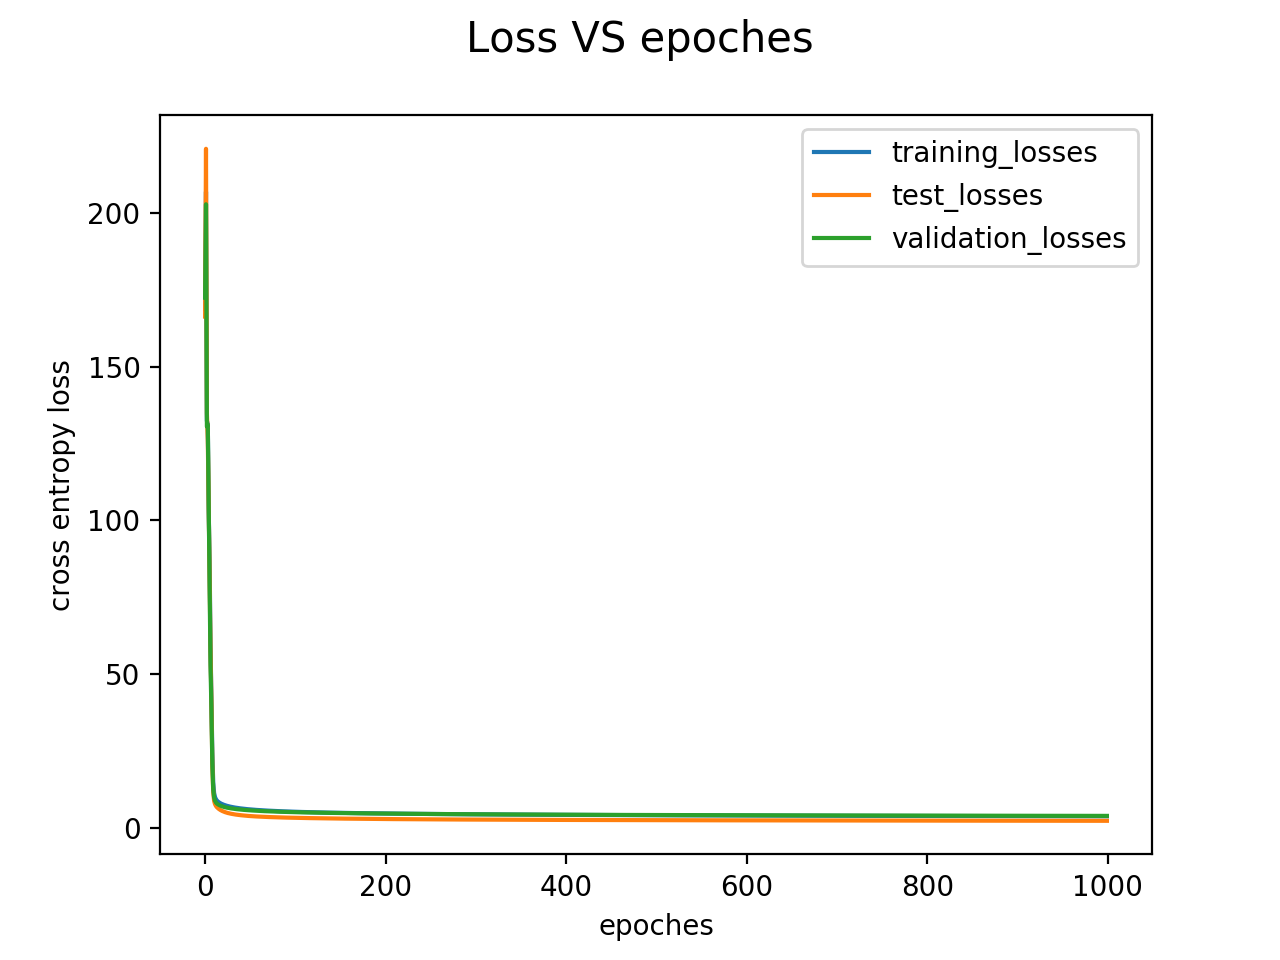
\includegraphics[width=2.5in]{../softmax/figs/loss.png}  }
		\label{fig: 11}
	}%
	\qquad
	\subfloat[The percent correct over the number of training iterations for the training, hold-out and test set.]{{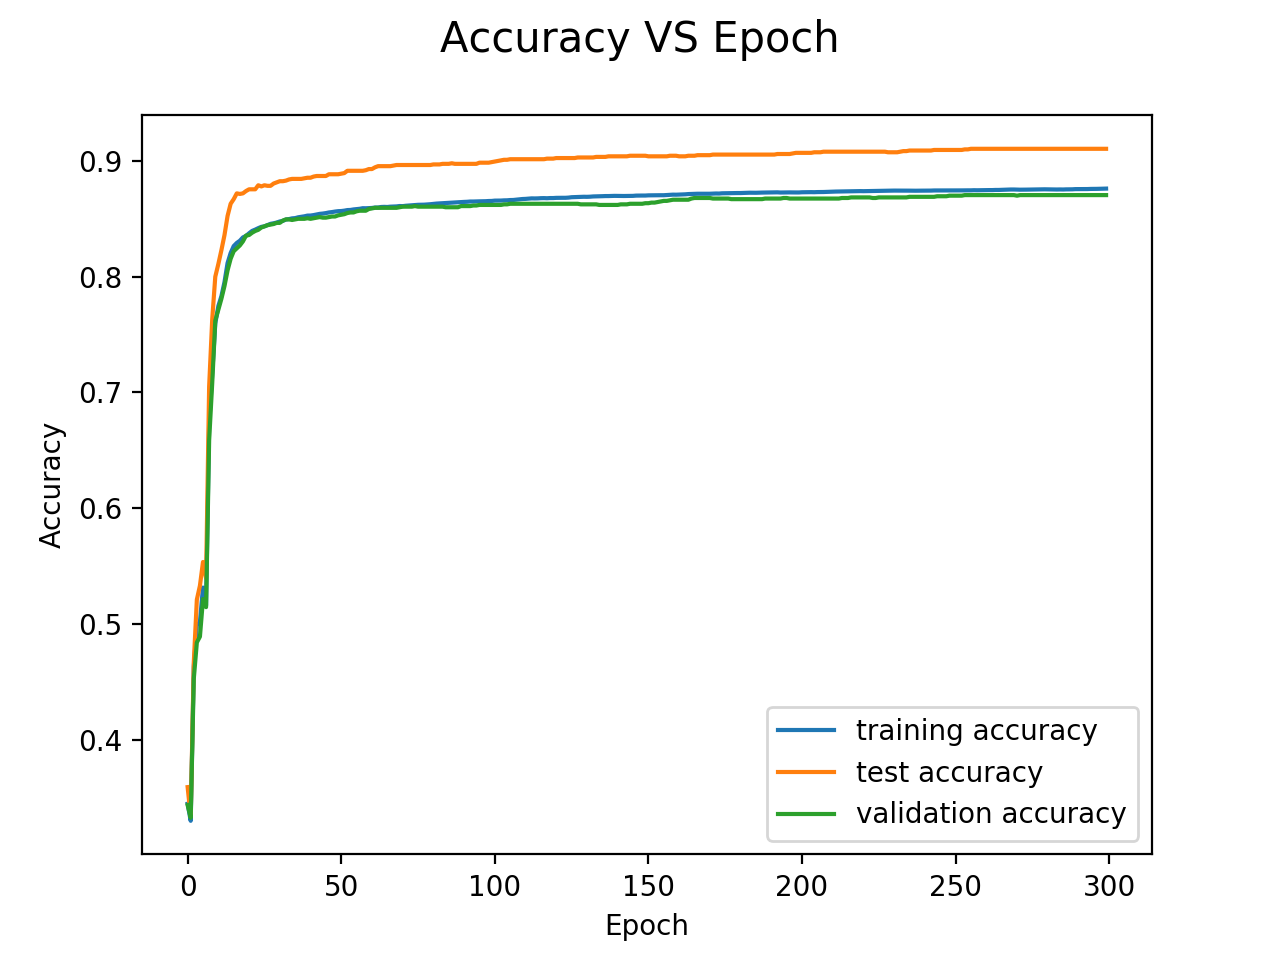
\includegraphics[width=2.5in]{../softmax/figs/accuracy.png} }
		\label{fig: 12}
	}%
	\caption{The performance of the algorithm over the number of training iterations. }%
\end{figure}

\begin{figure}[t]
	\centering	
	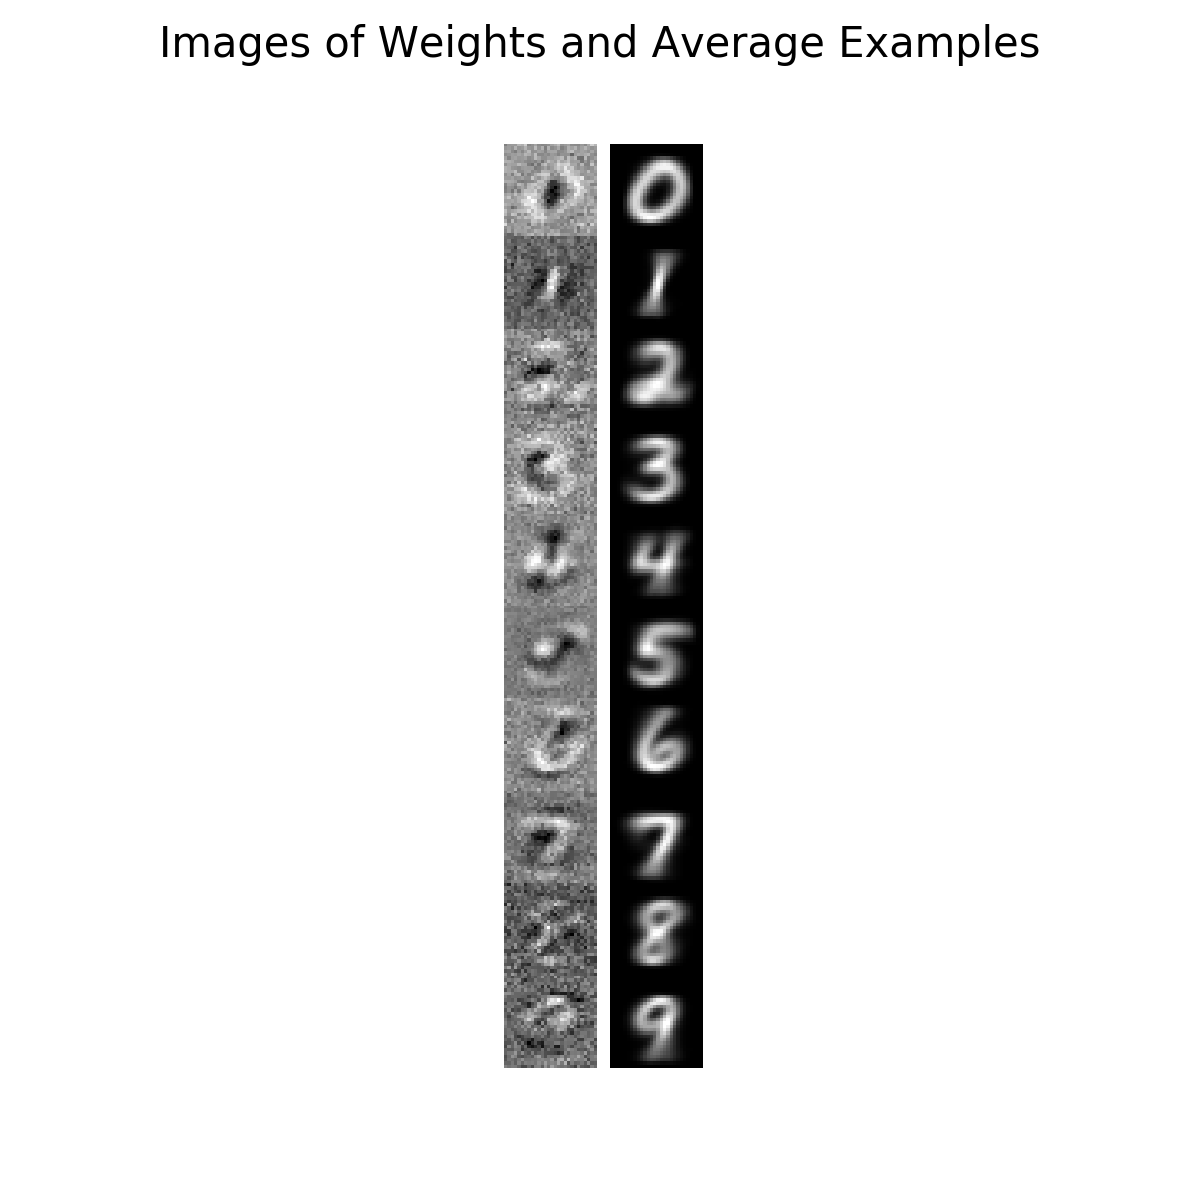
\includegraphics[width=2.6in,height=1.2in]{../softmax/figs/image_of_weights_and_digits.png} 
	\caption{Images of the weights and the average examples. The images in the first row are the images of the weights. The images in the second row are the images of the average examples.}
	\label{fig: 13}
\end{figure}

(b) In this experiement, we use $L_2$ regularization with $\lambda = 0.0001$. The figure is shown in Fig \ref{fig: 11}. Note that we use the sum of loss of individual data rather than the average one.


(c) In this experiement, we use $L_2$ regularization with $\lambda = 0.0001$. The figure is shown in Fig \ref{fig: 12}.

(d) We plot the results in Fig \ref{fig: 13}.


\subsection{Discussion}
From Fig \ref{fig: 11} and Fig \ref{fig: 12} and we can see that loss function went up and then  converges quickly and then becomes smooth. And the accuracy went up constantly accross diffrent datasets. The possible reason why the loss function went up in the first few epoches is that the learning rates maybe a little large to make to the loss function converge. But then after "annealing", we can see that the learining rates become reasonable enough to make the loss function to converge quickly to a local minimum. 

We tried setting the learning rate smaller initially but makes the algorihtm too slow to converge or just being stucked. If we set the initial learning rate to be 0.0005, the curve of the loss function becomes smoother, but after 300 epoches, the accuracy on the test set is about $88.9\%$ and is stucked. And if setting the learning rate too large initially makes the loss function up and down and makes it hard to converge. And we also see that there is no overfitting occurs. One possible reason for this is that the impact of the regularization. Another one is that the algorithm correctly learns the pattern underlying the data at hand.


From Fig \ref{fig: 13} we can see that the image of the weight and the corresponding image of the average digit is similar. The reason is that we classify the images based on the inner product of the pixels with the weights as we can see from the function below,

\begin{equation}
y_k^n = \frac{\exp{( w_k^Tx^n)}}{ \sum_{k'}\exp{(w_{k'}^Tx^n)}}
\end{equation}
So for an image belongs to class $k$, we want our model to output a large $y_k$ which indicates with a high probability that the image will belong to class $k$, we should make $w_k^Tx^n$ as large as possible. And the inner product is maximized when the angle between the weight and the image is zero. so we see that the image of the weight and the corresponding image of the average digit is similar.


\section{Summary}
In this work, we successfully derived and implemented logistic regression (binary classification) and softmax regression (multi-class classification) for handwritten digit classification problem from scratch and achieved roughly $98\%$ classification accuracy. We also embedded regularization to prevent overfitting so that the model generalized well to the unseen test examples. Through rigorous experiments and analysis, we can systematically tune the hyper-parameters and implement model selection by looking at the error on validation set. 

\section{Contributions}
\textbf{Shilin Zhu} did all the derivations, implementation codes, experiments, analysis of logistic regression part in this report (Section 2). 

\textbf{Yunhui Guo} did all the derivations, implementation codes, experiments, analysis of softmax regression part in this report (Section 3). 

Both Shilin Zhu and Yunhui Guo implemented both logistic and softmax regressions for own study purpose. Three discussions and pair programming were made before submitting this report.

\subsubsection*{Acknowledgments}

We would like to thank Prof. Gary Cottrell and all TAs' efforts in preparing and grading this assignment.

\subsubsection*{References}

\small{
[1] Bishop, C. M. (1995). Neural networks for pattern recognition. Oxford university press.

[2] Y. LeCun, L. Bottou, Y. Bengio, and P. Haffner. "Gradient-based learning applied to document recognition." Proceedings of the IEEE, 86(11):2278-2324, November 1998.

\section{Code}

\subsection{Logistic regression}
\begin{lstlisting}[language=Python]
%matplotlib inline
import numpy as np
import matplotlib.pyplot as plt
\end{lstlisting}

\subsection{Softmax regression}


\end{document}
